\chapter{PCB design}
\TODO{} introduction that mentions why we designed our own PCB (small device that can be contained in splashproof case + lots of peripherals + attaching to a moving horse requires extra stability).


\section{Schematic}
The schematic and layout were designed using CadSoft Eagle software version 6.1.0 It is not considered to be the most user friendly software in terms of the usage interface, but is fairly simple and straightforward. Furthermore, the user community is very large, therefore it is possible to find various component footprints already made by others to be used in the design. This decreases the overall time required to make a PCB design. Nevertheless, as we were using very specific components  (ANT, GPS, etc.) a footprint for them had to be designed manually by consulting the datasheet. 

\begin{figure}
\centering

\includegraphics[width=0.8\textwidth]{Images/dummy}
\caption{Block Diagram: Parts}
\label{fig:block_parts}
\end{figure}

\subsection{Power conditioning}
The power conditioning circuitry consists of two stages. First stage incorporates a constant current constant voltage single cell Lithium Ion battery charger centered around a ADP2291 chip from Analog Devices.  The second stage is a low dropout voltage (LDO) regulator based on a ADP1706 chip from the same manufacturer. For schematics see \TODO{Ref }Appendix X. 


\subsection{Battery charger}
The input voltage of the charger is in the range of 5 to 12V, therefore no power supply providing higher voltage than this is allowed to be used. D1 acts a reverse voltage protection diode in case the power supply is connected with a reversed polarity to the board. In case this ever happens it will not cause any damage to the components. 

C4 and C16 capacitors are used to filter out the noise that might come from the power supply. The chosen values of 820uf and 0.68uf are sufficient for this purpose. Resistors R2 and R6 placed in series with a battery provide current measurements for the charger. Hence, the charging current is adjusted by changing the R2 and R6 resistor values, that is currently set to 750mA. Internal LED driver is used to indicate the charging status of the battery. Charge status LED1 is ON when the battery is charging. Transistor Q1 acts as a pass device which provides a charging current to the battery. It was chosen with a reserve in parameter specifications. The device can handle continuous collector current of 3A and has a $V_{ceo}$ of 60V. This enables the device to function properly not only in the current setup but in a scenario when a higher current is required for faster charging. As a driver requirement the transistor has to have a certain minimum PNP beta (hfe coefficient), which for current configuration has to be no less than Imax / 40mA, where 40 mA is the base drive current and Imax is the charging current. This gives us the minimum beta of 18.75 that the transistor has to have. The chosen one has an hfe of 80 at collector current equal to 1A. 

In order to keep it from overheating a thermal protection is used by utilizing the NTC1 thermistor. This enables the charger to monitor the temperature of a pass device and decrease the charging current accordingly. Shutdown temperature of the charger is set internally to 100C. 

The charger works in step-by-step sequence illustrated by diagram \ref{fig:charger_sequence}:

\begin{figure}
\centering

\includegraphics[width=0.8\textwidth]{Images/dummy}
\caption{Battery charging sequence}
\label{fig:charger_sequence}
\end{figure}

\begin{itemize}
\item \textbf{Shut-down:} If the input voltage is lower than 3.8V the charger is in the shut-down mode. Power consumption from the battery is 1uA.
\item \textbf{Pre-charge:} When a voltage higher than 3.8V is detected at the input of the charger the charger checks the voltage across the battery and enters a pre-charge state if the battery voltage is lower than 2.8V. In this stage the maximum supplied current is 75mA. In cases where battery is deeply discharged and measures less that 1.5V the supply current is set to 150mA. 
\item \textbf{Fast charge:} If the voltage is higher than 2.8V the charger enters a full current fast charge mode which continues until the battery voltage reaches 4.1V 
\item \textbf{End-of-charge:} The charging current is reduced as the battery reaches its full capacity and once this current is less than 75mA an end-of-charge mode is initialized. 
\end{itemize}

Capacitor C6 determines the time of all operation modes. The ratio between the fast charge mode to pre-charge and end-of-charge is always 1/6. Given the capacity of our battery is 2200 mAh time required for it to fully charge with current settings is 2.9 hours. Therefore a timeout of 3 hours for fast charge mode is sufficient. C6 capacitance is calculated from the following formula $Ct = tchg *  1uf / 1800$ and is equal to 0.1 uf. The pre-charge and end-of-charge modes timeout in 30 minutes. Time limit of the fast charge mode is required as a precaution in case the battery fails to reach end-of-state mode for any reason.


\subsection{LDO regulator}
The LDO regulator takes in the provided voltage by the battery and outputs a fixed value of 3.3V required to power all on-board devices. Decision to use this type of regulator was made from the fact that the difference between input and output voltage is very small. Therefore, using a traditional linear regulator in this case is not an option. Our chosen device has a maximum dropout voltage of 55mV at 100mA output current. This figure increases to 345mV at output current of 1A respectively. The latter dropout will never be achieved, as in the worst case scenario when all peripherals are operational the maximum current consumption will be \TODO{check:} datasheet GPS, ANT, Xbee SD card + MCU 9.6mA
 all peripherals combined will hardly ever pass the 100mA current consumption point.
 
This LDO regulator was designed for operation with small value ceramic capacitors for space saving applications. Nevertheless, using a larger value output capacitors improves the transient response. Hence, as space is not an issue a value of 150uF was chosen. The regulator has a built in accidental short circuit protection. If for any reason the output becomes shorted, the regulator will conduct the maximum amount of 1.5A current into the short, increasing the junction temperature to critical level and triggering the thermal protection as a result turning off the output. 

A soft start function is implemented by connecting the C3 capacitor to ADJ pin of the regulator. This ensures a gradual output voltage ramp-up. The ramp up time is calculated using the following formula $T_{ramp-up} = 0.8V × (C3/1.2uA)$ Tramp-up represents the time it takes for the output to reach 90\% from 0\%. In current configuration where the value of C3 is 10nf the ramp-up time is 6.67 ms.

To insure a stable power supply to all components organic solid capacitors with conductive polymer (OS-CON) are used. Their benefits are discussed in 
\href{http://www.capacitorlab.com/capacitor-types-polymer/}{capacitorlab}  and  \href{http://www.capacitorsplus.com/whatis.htm}{capacitorplus}


\subsection{MCU}
As was mentioned earlier the MCU used for the project is EFM32GG332 based on ARM Cortex M3 core with a 1024KB of Flash and capable of running at a 48MHz speed. The chip has several clock sources and different crystal oscillators are used to generate that clock. XT1 is a high speed oscillator (HFXTAL) rated at 48MHz and running in a fundamental mode. XT2 is a low frequency oscillator (LFXTAL) rated at 32.768KHz and is produced by MEMS processing technology. This oscillator is used for peripherals running in low energy modes and operates in fundamental mode as well. The MCU will not work with a high speed oscillator that is specified to operate in an overtone mode. To insure that the crystal operates correctly, it has to have a certain load capacitance, in our case for XT1 this is 18pF and for XT2 it is 7pF. 

In case there is a need to reset the MCU it can be done by using the S1 global reset button. Capacitor C14 is used in parallel with the switch to implement a hardware de-bounce function. 

A standard approach for decoupling is used. One large capacitor C2 rated at 150uF is used for the whole system with 0.1uF C7-C12 capacitors used to decouple separate power pins. In our design we are not using ADC of the MCU; therefore it was not necessary to separate the digital and analog power domains. Separation is usually done to ensure better isolation and noise suppression between the power domains.


For programming and debugging the custom made PCB a debug interface consisting of clock input (SWCLK), data in/out lines (SWDIO) and serial wire output (SWO) had to be exposed. An external development kit was used to program/debug the PCB. By supplying the power to the PCB from the development kit via VMCU pin it was possible to measure the current consumption of a target with an Energy Aware profiler.

\TODO{Integrate with Monit Devs}

\subsection{I2C devices}
The TMP006 MEMS sensor from Texas Instruments was chosen for its ability to measure the temperature without the need of making a contact with an object. The measurement is done by allowing the thermopile to absorb the IR energy emitted from an object and based on the thermopiles voltage change determine its temperature.

Temperature sensor uses SMBus for transmitting transmit the data. The address of the device on a bus is set to 1000000 by grounding ADR0 and ADR1 pins. DRDY pin indicates whether the data is available to be read by the MCU and requires a pull-up resistor in order to operate correctly. Decoupling of the sensor is performed using a 22uF OS-CON and a 0.68uF plastic film capacitors.

The I2C bus is shared with an accelerometer. As this is not the only mode the accelerometer can operate the I2C mode had to be set by pulling the CS pin high. By setting the SDO/ ALT ADDRESS pin to high the accelerometers address becomes 0x1D on the bus. No pins are left floating in order to prevent leakage currents. Hence the Reserved\_3 pin is connected to +3.3V and Reserved\_2 together with Reserved\_1 are grounded. Optionally they can be left floating. 
The device can operate in several power supply modes. In this particular design it operates in a single supply mode, where VS is connected together with VDD/IO. Decoupling is performed for both of the pins using two 0.1uF ceramic capacitors. In addition to that a 22uF OS-CON is used at the VS pin to minimise the digital clocking noise.

\subsubsection*{ZigBee}
\TODO{}


\subsubsection*{ANT}
\TODO{}

\subsubsection*{GPS}
This module requires two power supplies, the first one VCC is used for digital parts and I/O and the second one VBAT is used for non-volatile back-up block. By default GPS does not have low energy mode that can be switched on demand, it does go into low energy mode automatically once it has acquired the satellite positions and collected the Almanac data. In normal operation mode GPS typically consumes 115mW of power which translates to 35mA of current draw from the battery. Nevertheless, this figure can rise up to 40mA. Power consumption drops to 75mW (22mA current draw from battery) once the GPS has finished with the cold start. This figure is still high. Power supply can be switched off for the VDD block if the navigation is not needed. This will enforce the GPS to enter the backup mode. The power then will be drawn from VBAT which is used for keep the collected satellite data in RAM. This will ensure a fast TTFF (time to first fix) once power on VDD is re-applied again. Power draw in this mode is in the region of 15uW (4.54uA).

The PPS (pulse-per-second) output is not used in the design as it is only required for timing purposes. 

For decoupling purposes a 0.1uF ceramic capacitors are used for both power pins with an addition of 22uF OS-CON for the VCC.

\subsubsection*{MEMS Microphone}
\TODO{}


\section{Layout}
\TODO{}


\begin{figure}[!htb]
\centering
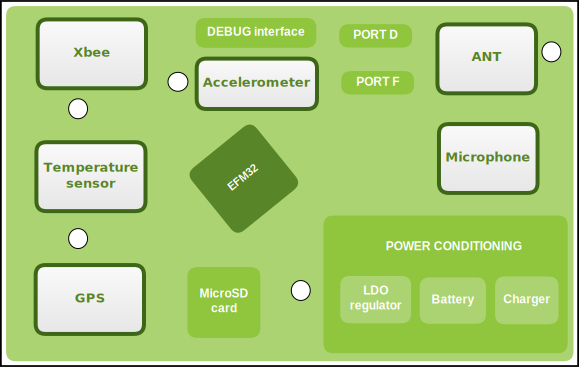
\includegraphics[width=\textwidth]{Images/board_layout}
\caption{PCB board layout}
\label{fig:board_layout}
\end{figure}

When positioning the components on the PCB some considerations had to taken into account. These are going to be discussed step by step starting with the power conditioning circuitry. 

The pass transistor Q1 used in the Charger generates a lot of heat, according to the calculation it dissipates \TODO{calculate} of power. In order to keep a low profile board the PCB itself acts as a heatsink. The pad of the transistor that draws away the heat from the crystal cannot be connected to the largest copper area of the board - GND, as the pad is internally connected to Vdd. Therefore a dedicated area was left for that purpose and thermally isolated from the neighbouring components. This also prevents the shortening of their lifespan. Multiple vias are used to connect the upper layer of copper with the bottom one making the heat dissipation more efficient. In case of overheating the NTC1 should tell the charger to decrease the current passing through the transistor lowering the power dissipation. Hence, the NTC1 was placed as close as possible to the transistor and was surrounded by the copper heatsink.

The LDO regulator has a SOIC package with an exposed pad underneath it. This is done to dissipate the generated heat directly into the board. The pad is internally connected to GND and in this case it was unnecessary to make dedicated heatsink area for this chip. As with the Multiple vias connect the upper and bottom layers of the PCB to promote better heat transfer.

Temperature sensor used in the project is one of the kind \TODO{}

The most practical way of placing the MCU is to put it in the center of the PCB. This enables the usage of short trace connections to the peripherals located on the sides of the board.

Decoupling capacitors are placed as close to the component power pins as possible. This applies to all ICs and modules used on the board without any exceptions.

\subsection{Soldering}
Soldering of components was done using several tools. This included a hot plate for reflow process and conventional tools for SMD components. Temperature sensor and an accelerometer were attached to the PCB using solder reflow as it was impossible to do solder them using conventional tools. An appropriate thermal profile had to be followed to prevent damage to the components. Both ICs have a peak soldering temperature of 260C but a slightly different thermal profiles, figure \ref{fig:temp_profile_optimal}(a) and figure  \ref{fig:temp_profile_optimal}(b) show the thermal profiles for temperature sensor and accelerometer respectively. 

\begin{figure}
\centering
\mbox{
\subfigure[]{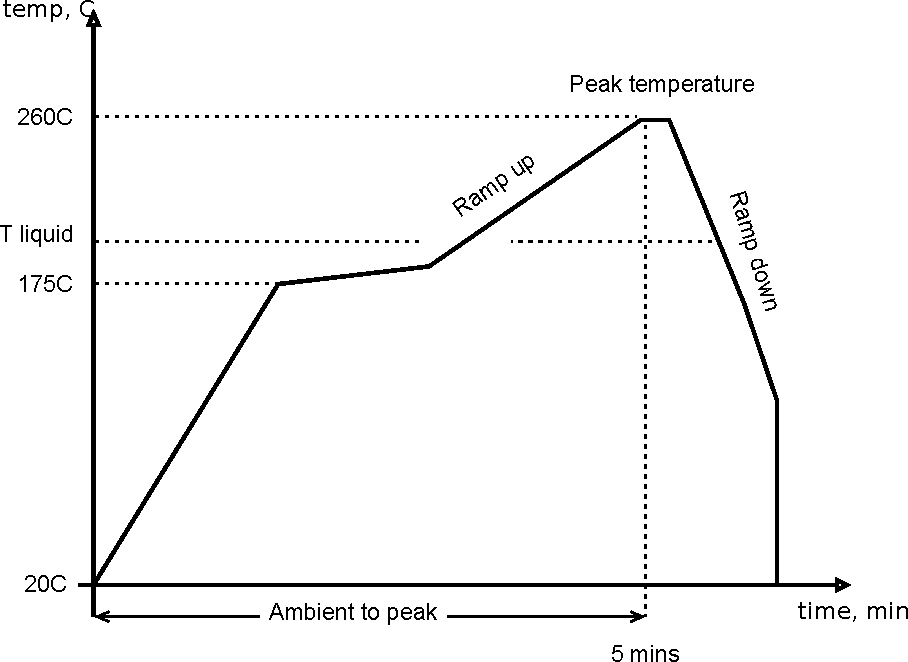
\includegraphics[width=0.45\textwidth]{Images/Thermal_profile_for_TMP006}}\quad
\subfigure[]{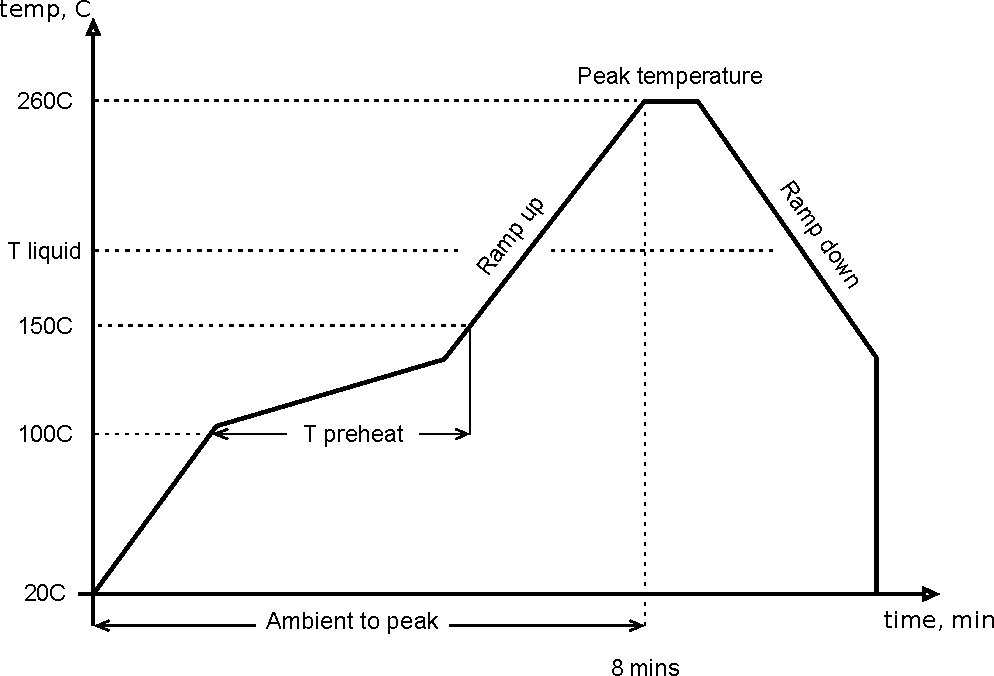
\includegraphics[width=0.45\textwidth]{Images/Thermal_profile_for_ADXL350}}
}
\caption{Optimal temperature profiles for soldering}
\label{fig:temp_profile_optimal}
\end{figure}

Ideally It should take no longer than 7 minutes to achieve the peak point from ambient temperature. This way the BGA package balls of temperature sensor would melt and produce a reliable contact to the PCB traces and accelerometer  without any risk of damaging the device. Nevertheless, the suggested profile for both ICs was impossible to achieve with the used hot plate as it only had an option of setting the end temperature point which took considerable time to reach. On average this time was 13 minutes as seen from the plotted thermal profile provided by the hot plate, figure \ref{fig:temp_profile_used}.

\begin{figure}
\centering
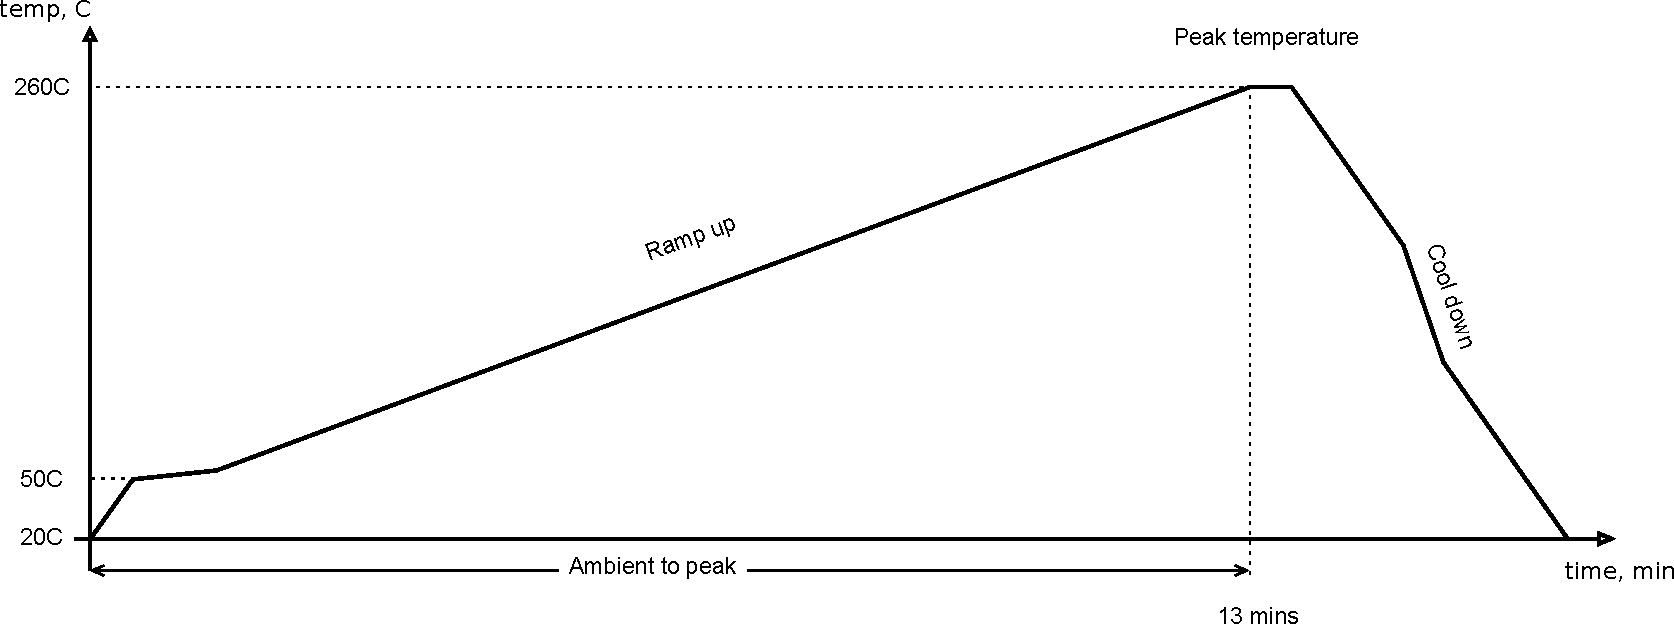
\includegraphics[width=\textwidth]{Images/Thermal_profile_used}
\caption{Used temperature profile for soldering}
\label{fig:temp_profile_used}
\end{figure}

It did increase the risk of damaging both of the components. Nevertheless, after the reflow they functioned as expected.
